
\newpage
\begin{appendices}

\section{Compiled code binaries}\label{annex:compilation}

% small intro
To perform the experiment on function renaming, the dataset used was a set of well-known open source programs:
% list of software used
\begin{itemize}
	\item Apache http server
	\item Filezilla ftp client
	\item Nginx http server
	\item OpenSSL library
	\item GlibC library
\end{itemize}


% symbols compilation summary and references
They were compiled from source using debugging options that make the final binary include the function names (also called symbols). Basically, each package or software had different options to include in the compilation command, but most of the times it required to include the -d for debugging option followed by some other indications. 


% example of symbols
Once the code is compiled with debugging information, the different functions or subroutines can be related to a function name that is listed inside the binary. Examples of function names are the following:

\begin{itemize}
\item aes\_encrypt\_cbc, which is highly informative of the purpose of the function, encrypting with AES algorithm using Cipher Block Chaining.
\item apr\_socket\_sendfile, which is again highly informative telling that it sends a file through a socket
\item \_zn9\_\_gnu\_cxx12\_\_pool\_allocice10deallocateepcy, others are not so informative or easy to understand, but at least it shows that it is handling memory pool allocations.
\end{itemize}

This will be the base on which a ruleset will transform each of the function names ( a total of more than 30000) into a small set of classes (8 for v1, 170 for v2 and 24 for v3 versions of the dataset)






\section{Feature extraction details}\label{annex:graph_from_code}


This annex will present the details of the implementation of the feature extraction from the dataset of assembly function code listings, used in the task of assembly function code classification.

\textbf{Graph of an assembly function code}

% compiled code binaries, machine code to assembly code
In this thesis, the tasks that classifies binary code functions takes advantage of programs that are prepared for reading and parsing binary files into human readable formats, using a programing language called assembler or assembly. However, a binary file is a file that contains bytes organized following a convention, or file format like PE or COFF, completely dependent of the operating system, but not assembler directives. The bytes contained in those file formats represent machine language code. This is not a problem as, per wikipedia definition, an assembly language (or assembler language), often abbreviated asm, is any low-level programming language in which there is a very strong correspondence between the program's statements and the architecture's machine code instructions. 


% Disassembler program, IDA free and how it works
For analysing a binary file, programs that convert the bytes of the binary file, that represent machine code, into assembler instructions are called disassemblers. For this thesis the selected disassembler program is called IDA free, which is a free version of the corresponding professional program IDA pro. This program reads the binary file bytes, according to the corresponding file formats, like PE for Microsoft Windows or COFF2 in Unix operating systems, and is able to interpret the machine code and translate it into assembler code instructions. There is a direct correspondence between machine code and assembler directives.

% IDA and python plugins
The selected disassembler program, IDA free, allows for executing scripts written in the programming language python. This scripts are run from inside its user interface to do tasks, like inspection and modification of the database of the binary code loaded.

% Plugin
The python script is ran as a script, also known as "plugin", inside the disassembler program (IDA free). It takes advantage of series of exposed interfaces or methods that read the database that contains the information of the disassembled binary file and its instructions. The procedure followed by the python script is to process all the lines of code of each function contained in the binary file. For each function or subroutine that the disassembler has detected, the python script will write 2 separate text files that contain the list of elements found as nodes and the list of relationships between them as edges, conveniently following a file format that the python package NetworkX can read and import into a NetworkX graph representation. 
The elements considered are all the types of elements that can appear in assembly code and that the disassembler detects: instructions, registers, memory addresses, immediate values, displacements and called functions. The edges represent relationships between them. For example, the instruction "mov eax, 0x0457AB" is related to the register "eax", the memory address "0x0457AB", as well as the previous and next instruction found in the code listing when following its execution flow. When the instruction is calling another function, for example "call another\_function\_address", an edge relating this instruction and the function another\_function\_address. 



\begin{figure}[H]
\minipage{0.5\textwidth}%
  \centering
    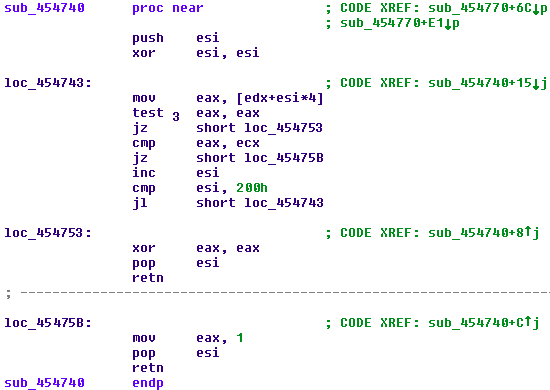
\includegraphics[width=0.9\linewidth]{img/code_graph02.png}
\endminipage
\minipage{0.5\textwidth}%
  \centering
    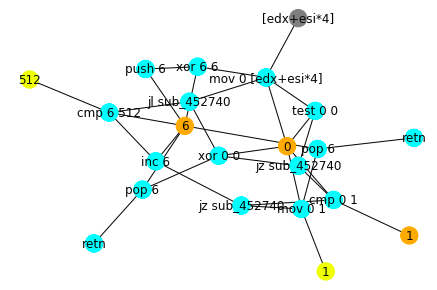
\includegraphics[width=0.9\linewidth]{img/code_graph01.png}
\endminipage
\caption{Assembler code transformed into a graph representation}\label{fig:code_graph01}
\end{figure}




% verification
Several assembly code functions are selected for testing the python plugin that generates the graph of the function code. The procedure is simple, the assembly code is printed as a code listing (each instruction is shown in assembly language in a separate line) like the disassembly program shows it inside its user interface. Then the contents of the file containing the description of the nodes, usually called function\_name\_nodes.txt where the function\_name part is replaced by the actual function name being analysed, and the file containing the set of edges joining nodes, usually called function\_name\_edges.txt where the function\_name part is replaced by the actual function name being analysed, are compared to the code listing to verify that every line of code, every register, memory address and the like is present in the nodes file, and every relationship between instructions, registers, memory addresses, called functions and the like is also present in the edges list file.


\begin{figure}[H]
\minipage{0.5\textwidth}%
  \centering
    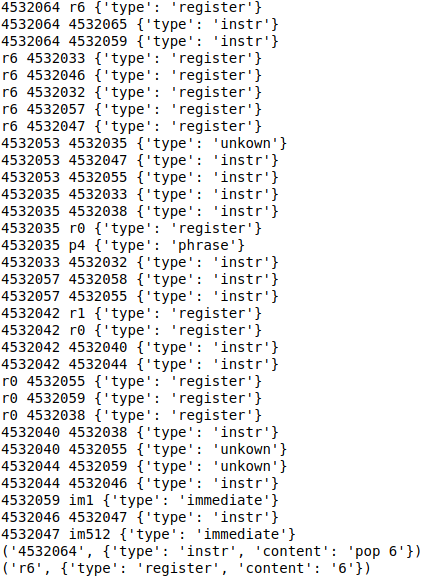
\includegraphics[width=0.85\linewidth]{img/code_graph03.png}
\endminipage
\minipage{0.5\textwidth}%
  \centering
    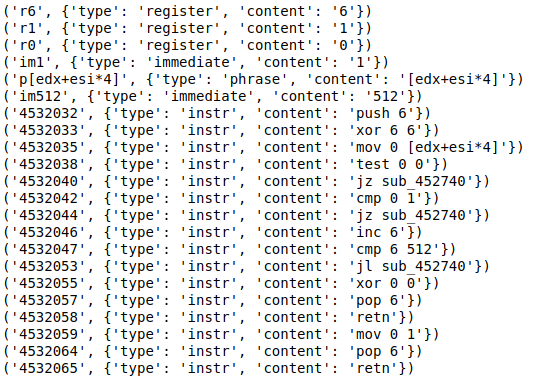
\includegraphics[width=0.95\linewidth]{img/code_graph04.png}
\endminipage
\caption{Edges and nodes list text files used to convert assembler code listings into graphs}\label{fig:code_graph02}
\end{figure}






\section{Labeling of the dataset}\label{annex:labels}


In this annex, a description of the process of labeling of the dataset is given.

The task of renaming functions in assembler code will be performed on a dataset of binaries that have been compiled with debugging information, that is with the so called symbols, which are the names of the functions or subroutines contained in the program. So, in the dataset every function keeps its original name.


The goal of the task is to predict a function name, in a more general way, by giving a name that describes or is a synonym of that main task performed by the function being renamed.  The current labels (the original names of the functions) are too specific. Thus, we need to assign as a label a name that is much more generalistic, in the sense that it indicates what is the main purpose of the function. The following steps have been followed.

First, a series of topics have been chosen:
\begin{itemize}
\item cryptographic
\item networking
\item graphical user interface
\item disk
\item data structures
\item memory
\item users
\item computation
\end{itemize}

Given the type of program binaries used as a dataset (network servers, clients and cryptographic applications), those topics cover the main functionalities of them.

Second, to be able to give a richer sense to the function names, a series of types of actions have been chosen:
\begin{itemize}
\item configure 
\item verify
\item save
\item delete
\item update
\item create 
\item get 
\item answer
\item read
\item write
\item send
\item receive
\item show
\item hide
\item start
\item stop
\item sync
\item parse
\item match
\item encrypt
\item data
\item file
\item compute
\item work
\end{itemize}

They have been chose based on the visual observation the real names in the dataset and by common sense also.

Third, 2 labeling strategies are created, one that consists of applying only the topic and a more comprehensive that assigns a topic and a task to a function. For example, the first labeling strategy may rename the function aes\_encrypt as cryptography, while the second strategy may rename it as cryptography\_encrypt. During the training of the models, those 2 labeling strategies will be compared. It is desirable that the second strategy is implemented over the first one, but the chance of success in this second strategy is lower as there are much more classes than in the second one. 

Finally, the labels have been assigned following very simple rules based on the real name of each function in the dataset and the number of appearances of each topic and task within it. The script uses the topics and tasks and their synonyms. It counts how many times each topic and each task appears in the real name of the function. The topic and the task that have the maximum number of appearances are assigned to the function. Two dataset are build, one with the first labelling strategy (assigning only the topic) and one with the second strategy (topic and task). The first dataset has 10 classes (9 + unknown). The second dataset has 170 classes. 

The final set of labels for each dataset version is shown below:

\begin{figure}[H]
\minipage{0.2\textwidth}%
  %\centering
    For the dataset v1:\\\\
   {\footnotesize
\begin{itemize}
	\item gui
	\item network
	\item disk
	\item cryptography
	\item datastruct
	\item memory
	\item process
	\item users
	\item computation
\end{itemize}
}
\endminipage
\minipage{0.45\textwidth}%
  
  For the dataset v2:\\

 \minipage{0.5\textwidth}%
  {\footnotesize
  \begin{itemize} 
    \item gui-hide
    \item gui-show
    \item gui-config
    \item gui-work
    \item gui-update
    \item gui
    \item network-send
    \item network-receive
    \item network-config
    \item network-save
    \item network-data
    \item network-file
    \item network-verify
    \item network-answer
    \item network-get
    \item network
    \end{itemize}
   }
   \endminipage
   \minipage{0.5\textwidth}%
   {\footnotesize
   \begin{itemize} 
    \item disk-work
    \item disk-read
    \item disk-write
    \item disk-delete
    \item disk-verify
    \item disk-parse
    \item disk-match
    \item disk

    \item cryptography-work
    \item cryptography-compute
    \item cryptography-send
    \item cryptography-encrypt
    \item cryptography-verify
    \item cryptography-config
    \item cryptography
    \item ...
%    \item datastruct-work
%    \item datastruct-config
%    \item datastruct%

    %\item memory-config
    %\item memory-work
    %\item memory-read
    %\item memory-write
    %\item memory-update
    %\item memory-delete
    %\item memory-create
    %\item memory-verify
    %\item memory



    %\item process-start
    %\item process-stop
    %\item process-create
    %\item process-update
    %\item process-delete
    %\item process-sync
    %\item process

    %\item users
    %\item users-create
    %\item users-update
    %\item users-delete
    %\item users-verify
    %\item users-config
    %\item users-save

    %\item computation
    %\item computation-work

	\end{itemize}
	}
   \endminipage
\endminipage
\minipage{0.35\textwidth}%
  
For the dataset v3:\\
\minipage{0.5\textwidth}%
{\footnotesize
\begin{itemize}
    \item gui-config
    \item gui

    \item network-send
    \item network-parse
    \item network-config
    \item network

    \item disk-file
    \item disk-read
    \item disk-write
    \item disk


    \item cryptography-encrypt
    \item cryptography-config
    \item cryptography
\end{itemize}
}
\endminipage
\minipage{0.5\textwidth}%
  
{\footnotesize
\begin{itemize}
    \item datastruct

    \item memory-config
    \item memory-read
    \item memory-write
    \item memory


    \item process-update
    \item process-sync    
    \item process-config  
    \item process

    \item users
    \item computation
\end{itemize}
}
\endminipage
\endminipage
\caption{Dataset labelling versions}\label{fig:labelling_versions}
\end{figure}










%During the training, some of the classes have been ignored due to the low frequency of appearance.







\section{Feature engineering in assembly code classification}\label{annex:feature_engineering}

Some of the machine learning models for classifying code functions in assembly (compiled binaries), make use of features that have been designed outside of the algorithm. It's the case of the code features, those related to aspects of an assembly function code like number of instructions or number of called functions, and the topological features of the graph of a function, those derived from the function's graph based on the relations between instructions, registers, memory addresses and other instructions. 
For the rest of the models of this task, the ones based on graph neural networks, there is no feature engineering, as they use the graph as an input to learning and prediction.

% HOW CODE FEATURES ARE EXTRACTED
The code features are aimed at summarizing or extracting relevant aspects of the underlying code. To this goal, counts of number of instructions, registers, memory addresses, function calls and the like are extracted from each assembly function code listing. The full assembly code listing is also extracted as a feature for models that use Bag of Words strategies. These features are simply obtained by reading the text files that list the nodes and the edges of the graph of the function, as the allow for recovering the basic elements on which the graph is constructed, the nodes, which are representations of instructions, registers, memory addresses and the like.
The list of features from code is the following:
\begin{itemize}
	\item  number of registers
	\item number of distinct registers
	\item number of instructions
	\item number of displacements
	\item number of immediates
	\item number of memory addresses
	\item number of functions called
	\item the list of words used in the code listing
	\item the list of words but replacing any register by the word register (and the same for memory addresses)
	\item a list of registers used
	\item a list of functions used
\end{itemize}

% TESTS CONDUCTED ON THE EXTRACTED CODE FEATURES
The code features extraction implementation is tested on several assembly function code listings, by comparing the counts of instructions, registers, memory addresses and the like versus those values extracted by the code that reads the text files that list nodes and edges of the graph of the assembly function.


% HOW TOPOLOGICAL FEATURES ARE EXTRACTED
The features that are derived from the topological aspects of graphs, like assortativity and clustering coefficient, are obtained with the implementation included inside the NetworkX Python library.

No testing of these topological features is performed, as the Python library NetworkX is used by a large community and has a great reputation. 
The list of the topological features extracted is the following:
\begin{itemize}
	\item number of nodes
	\item diameter of the graph
	\item radius
	\item average degree
	\item density
	\item node connectivity
	\item average clustering
	\item average shortest path length
	\item degree assortativity coefficient
	\item degree perason correlation coefficient
\end{itemize}




\section{Code repository}\label{annex:github}

The code and jupyter notebooks used in this project can be found at \href{https://github.com/presmerats/GNN-MThesis}{https://github.com/presmerats/GNN-MThesis} .

% explain the orgranization of the code repository
%doc
%src
%dataset
%girvan-newman
%graph-classification
%function-renaming

\end{appendices} 